

\section{Цель работы}
Целью данной работы является поиск звёзд, относящихся к определённому классу: звёзд типа Т Тельца (T Tauri звёзд).
Это предшественники звёзд, подобных Солнцу, а также планетарных систем. Поэтому их изучение очень важно для понимания процесса формирования Солнечной системы, её эволюции и образования планет. 

Как молодые звёзды, T Tauri обнаруживаются в областях звездообразования. Например, Т Тельца, по имени которой назван этот класс звёзд, расположена в молекулярном облаке Тельца (Taurus molecular cloud, TMC), где также находятся многие из известных T Tauri звёзд.

Критерии поиска кандидатов относятся к ультрафилетовой области спектра, отбор осуществляется на основе фотометрических измерений телескопа GALEX. Также используются данные в оптическом и инфракрасном диапазоне, взятые из каталогов 2MASS и UCAC4.

\section{Изучаемая область}

В данной работе изучается тёмная туманность, находящаяся в созвездиях Змея и Орёл (Serpens-Aquila Rift). Межзвёздная среда в ней находится в холодной фазе, то есть состоит из плотных и холодных облаков газа, в основном молекулярного водорода H$_{2}$. Именно из такого вещества формируются звёзды. Существуют исследования, подтверждающие, что в этой туманности происходит активное звездообразование \cite{park2012far}.

\begin{figure}[ht]
\center{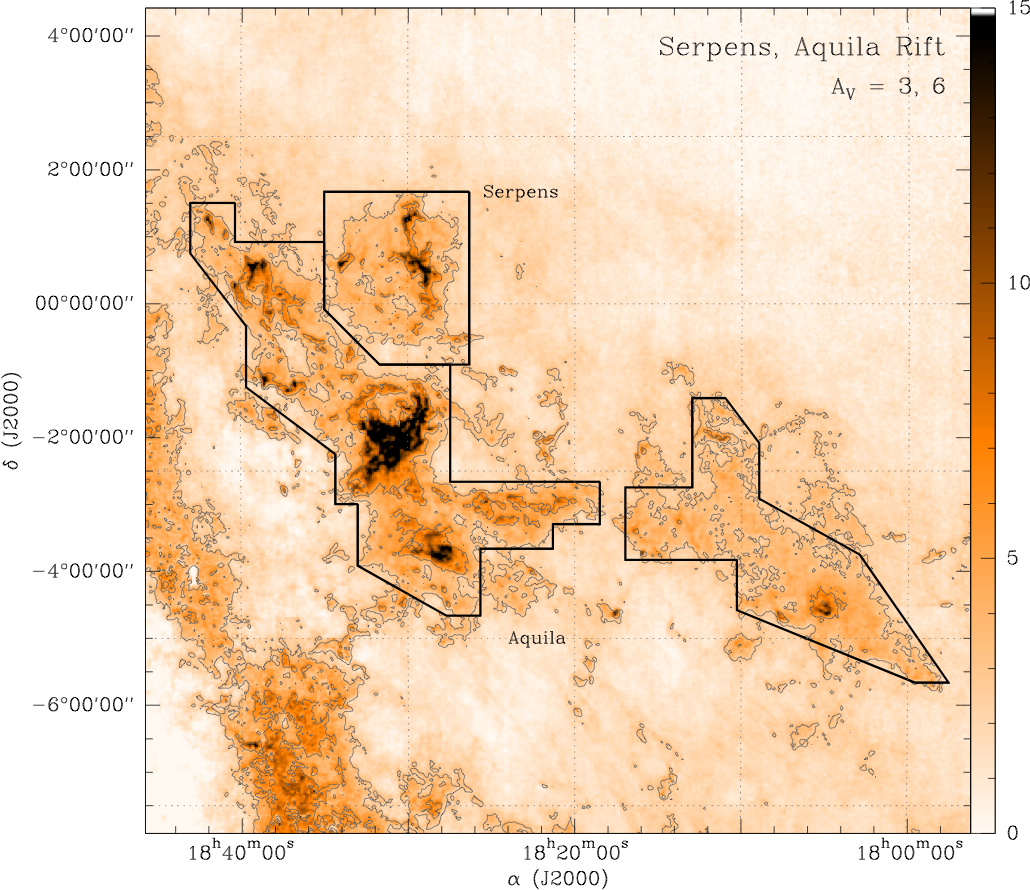
\includegraphics[width=0.6\linewidth]{gb_serpens.jpg}}
\hfill
\caption{Туманность в созвездии Змея. Карта межзвёздного поглощения в ближнем ИК, составленная С.~Бонтамом на основе данных 2MASS \cite{andreprobing}}
\label{fig:area}
\end{figure}


Расстояние до туманности оценивается по-разному. Та её часть, которая относится к созвездию Орёл, расположена на расстоянии 225$\pm$55 парсек от Земли. Область, относящаяся к Змее, несколько дальше. Согласно измерениям параллакса, проведённым на радиоинтерферометре VLBA, она находится на расстоянии 415$\pm$25 парсек \cite{park2012far}.

Несмотря на то, что исследуемая область известна наличием звездообразования, ни одна звезда в ней не идентифицирована как относящаяся к типу Т Тельца. Это связано с расположением туманности близко к галактической плоскости и недостатком наблюдений в нужных спектральных диапазонах.

Мы рассматривали область неба, для которой прямое восхождение лежит в интервале от 17.96 до 18.72, а наклонение от -5 до 5.5. Вторая часть туманности не рассматривалась из-за отсутствия необходимых наблюдений.

\section{Метод поиска}
T Tauri звёзды имеют несколько характерных спектральных особенностей, а именно избыток излучения в инфракрасном, ультрафиолетовом и рентгеновском диапазоне. Рассматриваются ИК, оптический и УФ диапазоны, но отбор осуществляется по фотометрическим данным, не требуя наличия спектров.

Алгоритм поиска аналогичен алгоритму, использовавшемуся в работе \cite{AIGdC2014galex} для молекулярного облака Тельца.

Исследование проводится на основе ультрафиолетовых фотометрических данных космического телескопа GALEX. По ним, а также по фотометриям UCAC4 в оптическом диапазоне и 2MASS в ИК диапазоне, строятся двухцветные диаграммы. Положения объектов на диаграммах сравниваются с положениями известных и подтверждённых звёзд типа Т Тельца для получения критериев отбора кандидатов.

Далее первичный список очищается от лишних источников заведомо иного типа, проводится анализ результатов и финального списка.

\section{Актуальность}
Звёзды типа Т Тельца интересны с точки зрения эволюции, как предшественники звёзд главной последовательности. Их изучение важно для понимания механизмов образования протопланетных дисков.


T Tauri звёзды эффективно исследуются в УФ области спектра, однако диапазон 115-300 нм недоступен для наблюдений с Земли.
После окончании миссии космического телескопа <<Хаббл>> единственным инструментом наблюдения в УФ диапазоне станет ВКО Спектр-УФ. Оснащённый трёмя спектрографами, он будет способен проводить спектральные измерения слабых объектов, вплоть до 17 звёздной величины \cite{malkov2011scientific}, что позволит подтвердить или опровергнуть принадлежность кандидатов к типу T Tauri звёзд.

Сам по себе список кандидатов в T Tauri звёзды нужен, чтобы определить объекты для наблюдения при дальнейшем поиске этих звёзд. Когда наблюдения проводятся космической обсерваторией и стоят дорого, важно выбрать звёзды, наиболее подходящие для изучения. И если научная задача состоит в измерении характеристик звёзд Т Тельца, наличие списка кандидатов весьма существенно.

Область молекулярных облаков в созвездии Змея пока слабо изучена в ультрафиолетовом диапазоне. Несмотря на то, что она известна как область звездообразования, в ней обнаружено совсем мало звезд типа Т Тельца, и ни одна из них не находится в изучаемой части неба.

